\section{Background}

\subsection{Edge computing}
\glsresetall%

Edge computing is a novel distributed computing paradigm, emerging from a need to overcome the drawbacks of offloading computation and data to the cloud.
Cloud computing, the reigning distributed computing model, allows users to access shared pools of resources such as servers, databases, and applications, over the internet~\cite{gai2012towards}.
These pools of resources are managed in a centralized manner by specialized providers, and users and businesses can access them on-demand, without having to invest in and manage infrastructure of their own.
Providers in turn employ economies of scale, providing these services by deploying massive amounts of computing power and storage capacity in specialized locations known as datacenters~\citationeeded.
These hardware resources are then further compartmentalized through the use of virtualization technologies such as \glspl{VM} and containers~\cite{gai2012towards}.

Through this design, cloud computing affords significant advantages to users.
As services are deployed in a centralized manner accessible over the internet, users can interact with their data and applications from anywhere in the world, from any device.
Thanks to economies of scale and virtualization technologies, the cloud is highly scalable;
services can be scaled simply by spawning more \glspl{VM}.
The specialized nature of cloud providers, the scale of modern datacenters, and the use of virtualization also make the cloud highly reliable.
When hardware fails, recovering is simply a matter of migrating the service container or \gls{VM} to an available compute node~\cite{endo2016high}.

However, the cloud is not suitable for everything, and presents important drawbacks and challenges for latency-sensitive and/or bandwidth-intensive applications.
In order to achieve the necessary economies of scale, cloud datacenters are designed to serve users distributed across vast geographical areas.
These installations are thus often located ``far'' from potential users;
for instance, at the time of writing, \gls{AWS} processes traffic from all of Scandinavia and the Baltic countries through a single datacenter in Stockholm~\cite{awsregions}.
This leads to prohibitively high latencies for both highly interactive immersive applications such as mobile \gls{XR} and for \glspl{CPS} and \glspl{NCS}~\cite{tolia2006quantifying,lagar2007interactive,satyanarayanan2009case,varghese2016challenges,shi2016promise}.
The former category requires \emph{motion-to-photon} latencies (i.e.\ time between input capture and feedback) below \SI{60}{\milli\second} for interactions to be perceived as fluid and responsive by the user~\cite{chen2017empirical}; the latter can require sub-\SI{10}{\milli\second} latencies, for instance in the case of vehicular safety systems.
Such latencies are unfeasible to consistently achieve with cloud computing~\cite{dang2021cloudy}.
On the other hand, as smart devices, appliances, and sensors become more and more ubiquitous, the network architectures of modern datacenters face increasing challenges to deal with the massively increasing volume of traffic~\cite{shi2016edge,wang2019towards}.

\begin{figure}
    \centering
    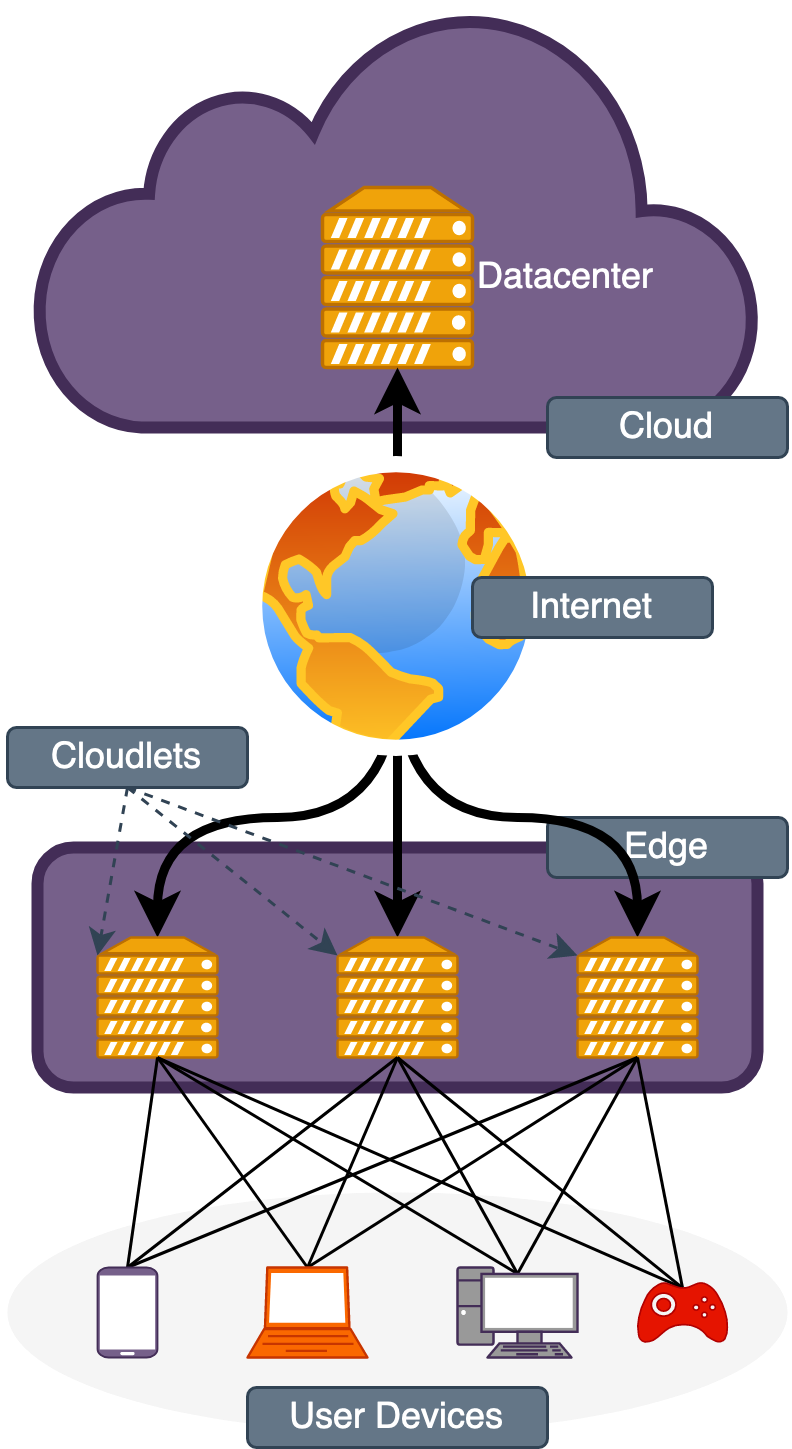
\includegraphics[height=30em]{figures/edgecomputing}
    \caption{%
        Conceptual design of edge computing.
        Micro-clouds (known as ``cloudlets''~\cite{satyanarayanan2009case}) are placed a at the edge of the network, a few hops away from end users.
        In other words, these cloudlets are located between users and the internet and the cloud.
    }\label{fig:edgecomputing}
\end{figure}

\medskip
Edge computing emerges as a potential answer to these challenges~\cite{satyanarayanan2009case,shi2016promise,shi2016edge,varghese2016challenges,satyanarayanan2017emergence,bittmann2017edge,wang2019towards}.
The foundation for this concept was laid by \citeauthor{satyanarayanan2009case}~\cite{satyanarayanan2009case} in\ \citeyear{satyanarayanan2009case}.
To tackle the prohibitively high latencies of cloud computing, the authors proposed an extension of the existing cloud computing paradigm with compute nodes at the edge of the Internet.
Instead of offloading computation to a datacenter potentially thousands of kilometers away, in edge computing it is offloaded to a micro-datacenter at the \emph{edge} of the network close to the user.
\citeauthor{satyanarayanan2009case} named these compute nodes \emph{cloudlets}, and envisioned them as featuring most of the key characteristics of cloud datacenters, such as multi-tenancy, virtualization of computing resources, virtually unrestricted access to energy, as well as limited scalability, all while being one or two hops away from the user (see \cref{fig:edgecomputing})
This built on previous work on \emph{cyber foraging}~\cite{noble1997agile,flinn1999energy,satyanarayanan2001pervasive}.
Cyber foraging refers to the extension and amplification of the capabilities of mobile and wearable devices by offloading computation and data manipulation to nearby infrastructure (as opposed to distant infrastructure such as the cloud).
This reduces energy consumption and allows for the deployment of otherwise unfeasible workloads on mobile hardware.

The architecture of edge computing offers several advantages, the primary being the significant reduction of latency.
Cloudlets can serve highly latency-sensitive and resource-intensive applications with extremely low latencies while still providing orders of magnitude more computing and energy resources than those present on mobile and wearable devices.
Another advantage is bandwidth reduction.
%By processing and aggregating data closer to where its needed, edge computing can significantly reduce the amount of traffic going to cloud datacenters.
A variant of edge computing called \emph{fog} computing, introduced by \citeauthor{bonomi2012fog}~\cite{bonomi2012fog} in\ \citeyear{bonomi2012fog}, concerns itself specifically with the distribution of computing power between the cloud and the edge for this purpose.
By aggregating, transforming, and filtering data at multiple levels in the network, fog computing aims to reduce the load placed on cloud datacenters by massive \gls{IOT} sensor networks~\cite{yi2015survey}.
Edge computing also presents opportunities for increased data security, privacy, and integrity, by keeping it geographically close to its origin and by allowing for anonymization through denaturing and local aggregation before offloading to cloud services~\cite{satyanarayanan2017emergence}.

Finally, in later years, edge computing has been paired with novel mobile networking standards such as 5G~\cite{hassan2019edge,pham2020survey,wan2020efficient}.
This combination is often referred to as \gls{MEC}, and has the potential to enable unprecedented use-cases requiring stringent latency bounds and high bandwidths.
Two examples of such applications, of relevance for the present work, are \acl{WCA}~\cite{ha2014towards,chen2018application,wang2020scaling,chen2017empirical,chen2018application} and \aclp{NCS}~\cite{sasaki2016vehicle,wang2018bandwidth,wan2020efficient}.
These applications had been hitherto inviable to implement due to the limitations of cloud offloading in mobile and wearable contexts, but have now become a practical reality thanks to \gls{MEC}.
We will discuss these in depth in their respective sections, \cref{background:wca} and \cref{background:ncs}.

\subsection{Emulation and simulation}

The terms \emph{emulation} and \emph{simulation} are often used interchangeably.
However, although both terms refer to methods of imitating and modeling systems, they are distinct in their goals, methods, and applications.

Emulation refers to the process of reproducing or mimicking the observed behavior of a system through another system, 
with the ultimate goal being the recreation of behavior that matches the original system as close as possible.
Emulations run in \emph{real time}, and can thus interact with real environments;
in turn, this means that emulations can be used to replace subcomponents of larger systems for research or benchmarking.
This method does not aim to model the original system, nor aim to understand its underlying behavior.

Simulation, on the other hand, is the process of modeling a system to study its behavior through the creation of a mathematical or logical model of the system.
The model can then be adjusted to simulate and better represent the original system in different scenarios and conditions.
Simulations run in entirely virtualized environments, and are not beholden to any real-time constraint.

Finally, these approaches differ as well in the level of accuracy each of them affords.
While simulation only attempts to approximate the behavior of the system in a given context, emulation aims to represent as close to a perfect copy of the observed behavior of the system.
The former is therefore employed when a general understanding of the system is sufficient, while the latter is used when precision is required.
However, thanks to its real time constraint and high degree of realism, emulation is typically more resource-intensive than simulation.
This means that emulation requires more processing power, memory, and storage space than simulation.

\subsection{\glsfmtlong{XR}}\label{background:xr}
\glsreset{XR}
\glsreset{AR}
\glsreset{VR}
\glsreset{MR}
\todo[inline]{Add some references}
\todo[inline]{Discuss tethered versus untethered}

\gls{XR} is an umbrella term used to refer to all immersive technologies that combine real and virtual environments, including technologies such as \gls{AR}, \gls{VR}, and \gls{MR}.
\gls{AR} merges digital content with the physical world, enhancing human perception and cognition through the overlay of virtual objects and information on top of the real environment.
This technology can superimpose tooltips, virtual \gls{2D} and \gls{3D} objects, or even full-fledged videos on top of what the user sees.
These overlays are most often presented to the user through wearable or mobile devices, such as smartphones or smart glasses (e.g. Google Glass), fitted with a camera to capture a real-time video feed of the physical environment and a display on which the augmented feed is presented.

\gls{VR}, on the other hand, takes it a step further and involves fully forgoing the real world, immersing the user in a fully digital, \emph{simulated} environment.
Due to its deeply immersive nature, \gls{VR} requires hardware components specifically designed for this task, the most crucial of which is the \gls{VR} headset.
The simplest type of such headset uses a pair of lenses to present an illusion of depth when looking through them at a small display.
More advanced types combine microdisplays, accelerometers, and headphones to provide a comprehensively immersive experience, where the user truly feels as if they are inside the virtual world.
Additionally, \gls{VR} systems often allow users to interact with the simulated environment through the use of instrumented gloves or special controllers, further increasing the illusion of immersion.

Finally, \gls{MR} combines elements from both aforementioned technologies.
As in \gls{AR}, \gls{MR} overlays virtual objects on the physical, real-world environment, while also involving the tools and techniques from \gls{VR} which allow the user to manipulate these.
In this way, \gls{MR} creates a hybrid environment where users can interact with both virtual and real-world elements simultaneously, resulting in an illusion of natural interaction between users and digital elements.

\medskip

Due to their ability to create immersive experiences for users and closely mimic and simulate real-life scenarios, \gls{XR} systems have found applications across a wide spectrum of industries and fields.
One of the most common uses of these technologies can be found in the domain of entertainment.
\gls{VR} allows users to become fully immersed in virtual experiences, including games, concerts, movies, making them feel almost physically present without having to leave the comfort of their homes.
Further, \gls{AR} and \gls{MR} allow for the merging of the virtual and real worlds, bringing entertainment to life in users day-to-day surroundings.
The popularity of this approach can be clearly seen in the explosive success of modern mobile \gls{AR} games such \citetitle{pokemongo}~\cite{pokemongo}.

\gls{XR} also presents tremendous opportunities for education and training.
Through the use of these technologies, students can get hands-on yet safe, simulated experience in a multitude of scenarios.
\gls{VR} is leveraged, for instance, in the training of new medical professionals, allowing students to learn anatomy and practice surgical procedures in realistic virtual environments.
On the other hand, \gls{AR} and \gls{MR} are employed in manufacturing, to train and assist technicians in highly specialized assembly lines.
Workers can receive real-time guidance through \gls{AR}-enabled headsets, improving accuracy and safety while controlling machine operations on the factory floor.
\gls{AR} can also provide augmented, step-by-step guidance for maintenance and repair of equipment, augmenting thus the capabilities of workers and the productivity of the workplace as a whole.

\subsubsection{\glsfmtlong{WCA}}

Of particular interest for this dissertation is a particular subset of \gls{AR} denoted \acf{WCA}, a technology designed to provide real-time support and guidance to individuals performing complex tasks in a plethora of domains.
Designed to be deployed on wearable devices, \gls{WCA} overlays digital information onto the real world and provides context-aware feedback to users, in order to assist and guide them in to efficiently complete a task~\cite{ha2014towards,chen2015early,chen2018application,wang2020scaling}.

These applications operate in a manner analogous to how \gls{GPS} navigation assistants guide users. 
The progress of the user is seamlessly and continuously monitored by the application, which provides relevant instructions and feedback only when these are needed.
The application follows the progress of the task in ``realtime'' by repeatedly sampling the state of the physical system, most commonly through video feeds.
Whenever the assistant detects a change in the context of the user, it provides a new instruction.
The application otherwise remains silent and out-of-the-way.

Originally motivated by assistive use-cases for individuals with reduced cognition due to illness, injury, or age, \gls{WCA} technology has been evolved to include the enhancement of the cognitive abilities of users in areas such as manufacturing, healthcare, and aviation.
Among the primary benefits of this technology is that it can help reduce the cognitive load on individuals performing complex tasks.
By providing real-time guidance and support, it can improve accuracy and speed of task completion, reduce errors and minimize the risk of accidents.
For example, a \gls{WCA} could help a technician performing maintenance on an aircraft by displaying relevant technical information about the aircraft parts and step-by-step instructions on how to perform complex specific repairs.

\gls{WCA} technology employs sensors, cameras, and other hardware in wearable devices to collect data from the environment and the user.
This data is then processed to interpret the data and provide relevant feedback.
As with many other categories of \gls{AR} applications, the computational complexity of the processing of the real-time input data makes it unfeasible to do on wearable devices.
The context-rich and latency-sensitive nature of \gls{WCA} inputs further makes this category of applications a prime candidate for offloading to the Edge.

Overall, \gls{WCA} is a promising technology that has the potential to revolutionize the way we perform complex tasks.
As the technology continues to evolve and become more sophisticated, it is expected to have a significant impact on many industries and improve the safety and efficiency of numerous processes.

\subsection{\glsfmtlongpl{NCS}}\label{background:ncs}
\glsreset{NCS}

\glspl{NCS} are a class of control systems that involve the integration of communication networks into traditional control systems.
A control system is a collection of devices or subsystems that work together to achieve a desired behavior or outcome of a physical system.
These systems are composed of
\begin{inlineenum}
    \item a \emph{plant}
    \item \emph{sensors}
    \item \emph{actuators}
    \item a \emph{controller}
\end{inlineenum}.
Plant refers to the physical system being controlled.
Sensors sample and encode the state of the plant and transmit it to the controller.
The controller processes these inputs, and generates control signals to be sent to the actuators, which modify the plant's behavior.
The overall goal of a control system is to regulate a process or a physical system to meet desired specifications or objectives, such as maintaining a constant temperature, tracking a set trajectory, or regulating the speed of a machine.

\glspl{NCS}~\cite{gupta2010networked} aim to enhance and extend the capabilities of traditional control systems by decoupling the controller from the plant, sensors, and actuators and interconnecting them with general-purpose \acs{TCP}/\acs{IP} networks;
see \cref{fig:csvsncs}.
This allows for remote monitoring and control, which enhances the reliability and safety of the control system, which is particularly useful in applications where real-time monitoring and control are critical, such as in industrial automation and transportation systems.
\glspl{NCS} also enable the integration of multiple control systems, as well as centralized control of multiple plants by a single controller.
This leads to enhanced scalability and flexibility, and allows improved coordination and collaboration among systems.
Furthermore, \glspl{NCS} provide greater access to information, as they enable the exchange of data and information between control components and systems, leading to more informed decision-making and improved performance.

\begin{figure}
    \centering
    \begin{subfigure}[t]{0.45\textwidth}
        \centering
        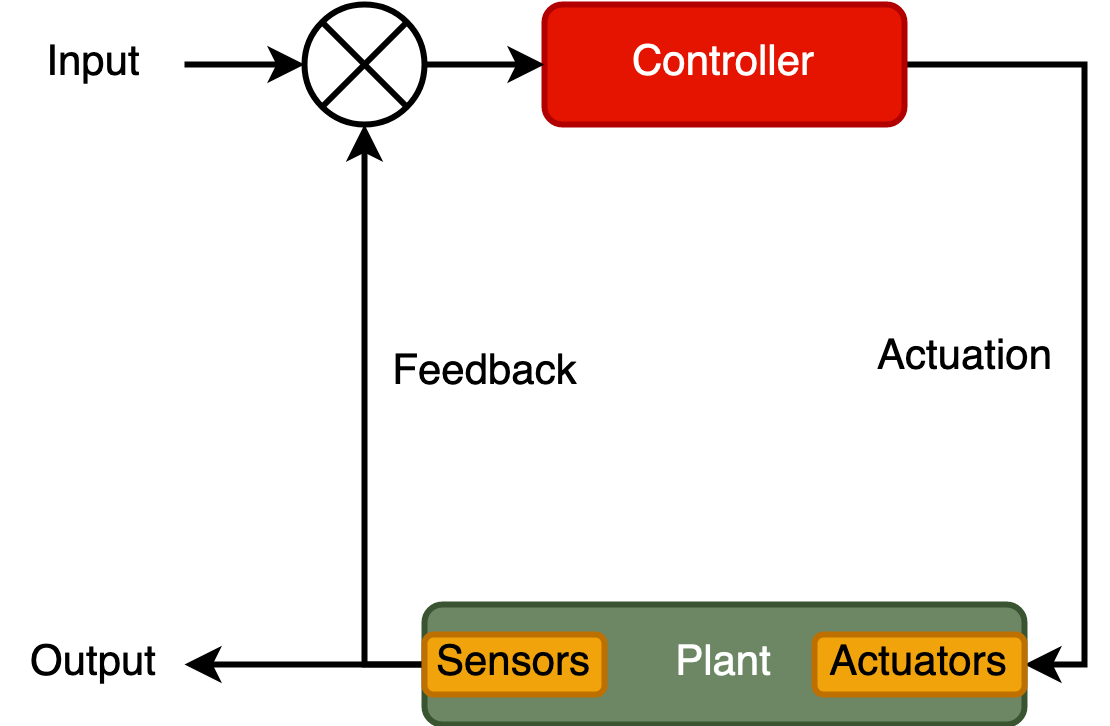
\includegraphics[width=\textwidth]{Figs/control_system}
        \caption{%
            Traditional control system.
        }
    \end{subfigure}%
    \hfill%
    \begin{subfigure}[t]{0.50\textwidth}
        \centering
        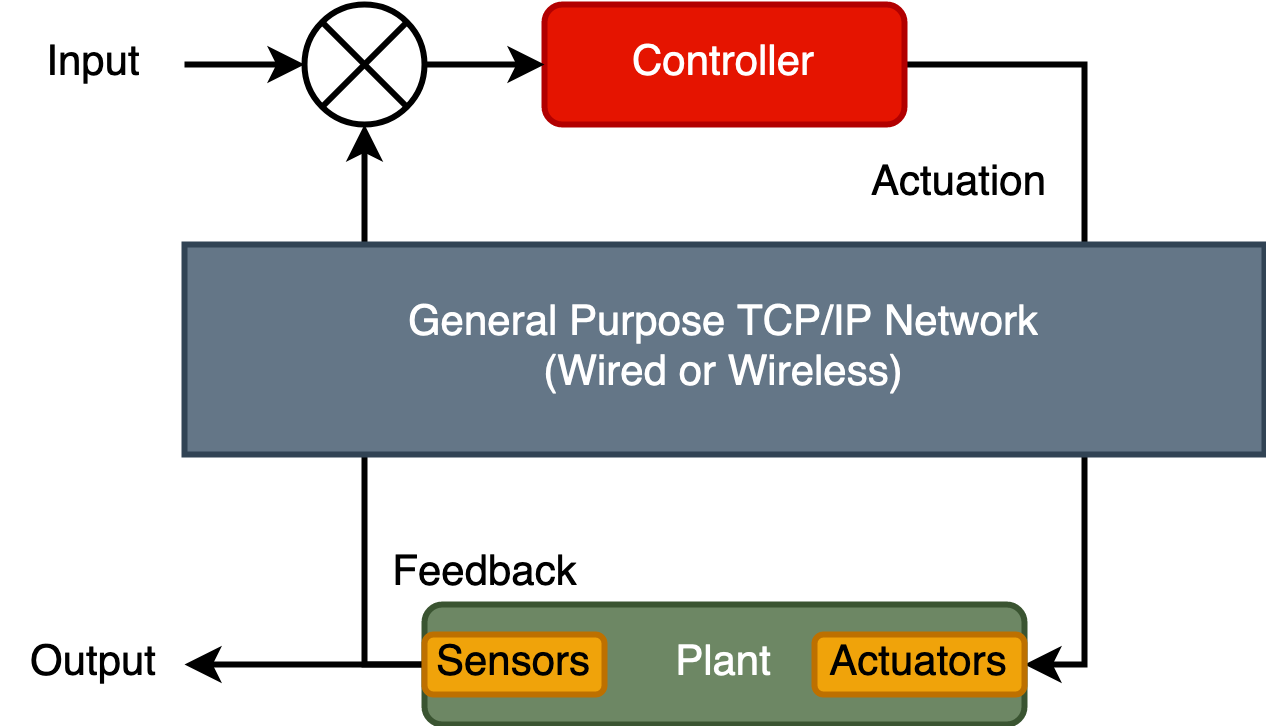
\includegraphics[width=\textwidth]{Figs/networked_control_system}
        \caption{%
            \acl{NCS}.
        }
    \end{subfigure}
    \caption{%
        Comparison between traditional control systems and \aclp{NCS}.
        In an \aclp{NCS}, controller and plant are physically separated and both actuation commands and sensor inputs are shared through a general purpose \acs{TCP}/\acs{IP} network.
    }\label{fig:csvsncs}
\end{figure}

\glspl{NCS} have become increasingly popular in recent years due to advances in communication and control technologies, as well as the increasing demand for real-time, remote, and distributed control.
They have found use in varied applications, such as industrial automation, transportation systems, and smart buildings, and some have attempted to leverage the cloud for centralized, distributed control in what has been called \emph{cloud control systems}~\cite{xia2015cloud}
However, depending on the physical system being controlled, \glspl{NCS} can have stringent timing and reliability requirements for communication that conventional cloud paradigms simply cannot meet~\cite{wan2020efficient}.
This has led their adoption to be limited mostly to industrial environments.
This is about to change, however, as with the advent of edge computing, paired with novel wireless communication technologies such as cellular 5G, consumer-grade \glspl{NCS} will be made possible.
These technologies will likely become the backbone of consumer-grade, widely-deployed \glspl{NCS}, enabling real-time capabilities through extremely low end-to-end latencies together with context- and locality-awareness.

\subsection{Emulation as a research methodology}
\todo[inline]{Rename?}
